\documentclass[conference]{IEEEtran}
\IEEEoverridecommandlockouts

\usepackage{cite}
\usepackage{amsmath,amssymb,amsfonts}
\usepackage{graphicx}
\usepackage{textcomp}
\usepackage{xcolor}
\usepackage{array}
\usepackage{booktabs}
\usepackage{url}
\usepackage{tikz}
\usepackage{float}
\usetikzlibrary{shapes.geometric, arrows.meta, positioning, fit, calc}

\begin{document}

\title{AirSketch: A Real-Time Gesture-Based Virtual Drawing and Control System Using MediaPipe and OpenCV}

\author{
\IEEEauthorblockN{Dr. Anita Harsoor, Hisham Khuram, Md Ahmed Raza Sofi, Mohammad Abdul Maaz Hanan}
\IEEEauthorblockA{Department of Computer Science and Engineering\\
P.D.A. College of Engineering\\
Kalaburagi, India\\
\{anitaharsoor, 3pd23cs050, 3pd23cs065, 3pd23cs070\}@pdaengg.com}
}

\maketitle

\begin{abstract}
Touchless human–computer interaction enables direct control of digital content through physical movement. This paper presents AirSketch, a real-time gesture-based virtual drawing system developed using Python, OpenCV, MediaPipe, and NumPy. A standard webcam captures hand movements, while MediaPipe detects hand landmarks and uses the index fingertip as the interaction point. A distance-based pinch gesture activates drawing and shape creation, while a five-sample moving average reduces cursor jitter. The system supports freehand drawing, erasing, geometric shapes, color selection, brush-size control, and canvas clearing. AirSketch uses a lightweight, deterministic approach without requiring depth cameras, gloves, or trained gesture classifiers. The paper discusses its architecture, interaction model, rendering process, implementation, and functional evaluation, along with limitations such as sensitivity to lighting and camera quality, single-hand operation, and limited gesture vocabulary.
\end{abstract}

\begin{IEEEkeywords}
hand gesture recognition, human--computer interaction, MediaPipe, OpenCV, virtual drawing, touchless interface, hand landmarks, computer vision
\end{IEEEkeywords}

\section{Introduction}
Human--computer interaction (HCI) has progressively moved from command-oriented interfaces toward interaction techniques that attempt to resemble natural human behavior. Hand gestures are particularly attractive because they can express pointing, selection, manipulation, and continuous motion without requiring the user to hold a physical controller. Vision-based gesture interfaces have consequently been studied for applications including assistive interaction, virtual environments, robotics, sign-language processing, and touchless control. Reviews of the field commonly describe a processing chain involving image acquisition, hand detection or segmentation, feature extraction, and gesture classification or interpretation \cite{qi2024,vuletic2019,rahman2020}. These studies also highlight a persistent trade-off: systems using specialized sensors or richer learned models may provide additional information, but they can increase hardware, computational, or deployment requirements.

The choice of sensing technology strongly affects the practicality of a gesture interface. Wearable approaches such as instrumented gloves can provide direct measurements of hand configuration, while depth cameras can supply three-dimensional information. Camera-only approaches, in contrast, can use hardware already available on many computers and therefore offer a lower barrier to experimentation and deployment \cite{rahman2020,qi2024}. Recent progress in landmark-based hand perception has made this approach substantially more practical. MediaPipe Hands introduced a real-time pipeline that combines palm detection with a hand-landmark model and estimates a 21-point hand skeleton from a single RGB camera \cite{zhang2020}. The resulting representation is useful not only for recognizing predefined gestures but also for constructing application-specific interaction rules from spatial relationships among landmarks.

Virtual drawing is a natural application for this type of interaction because the desired input is inherently spatial: a user's fingertip trajectory can be mapped to a two-dimensional drawing surface. Existing air-canvas prototypes have demonstrated the feasibility of combining OpenCV and hand tracking to draw without a mouse or stylus \cite{vasavi2022,swathi2024}. However, a drawing application requires more than fingertip tracking. It must distinguish between movement that should create a stroke and movement that should manipulate the interface, provide stable interaction despite small tracking fluctuations, support tool selection, and provide feedback while an object is being created. Gesture-based interface research also shows that gesture selection is not purely a recognition problem; the appropriateness and usability of the gesture vocabulary are important design considerations \cite{vuletic2019}.

AirSketch addresses this application-level problem with a deliberately compact interaction model. Rather than training a new neural classifier for each drawing command, the current implementation uses MediaPipe's landmark output and deterministic geometric rules. The index fingertip provides the interaction coordinate, while the distance between the index and middle fingertips determines whether the interaction is active. This design makes the control logic explicit and easy to inspect. It also separates perception from application behavior: MediaPipe supplies hand geometry, while AirSketch decides how that geometry controls drawing and interface operations.

The present work differs from the earlier version of the project documentation in an important respect. The current implementation is a Python/OpenCV desktop application rather than a browser-based React application. Its dependencies are limited to MediaPipe 0.10.21, OpenCV 4.10.0.84, and NumPy 1.26.4, and the interaction logic is implemented directly in Python \cite{repo}. Therefore, this paper is based on the current implementation rather than reusing technology claims from the previous project paper.

The main objectives of this work are: 1) a webcam-based virtual drawing system using MediaPipe hand landmarks; 2) Enhance accessibility by enabling users with physical limitations to
interact without traditional input devices 3) Demonstrate the practical use of AI-driven human–computer interaction
systems 4) Provide an interactive and user-friendly interface with
features such as drawing, color selection, erasing, and
canvas clearing. The goal is not to claim a new hand-tracking model, but to demonstrate how an established landmark detector can be integrated into a practical touchless drawing system with a small and interpretable control layer.

\section{System Design and Methodology}

\subsection{Design Requirements}
The system was designed around five functional requirements. First, interaction should be possible using a conventional webcam without a wearable device. Second, the system should operate continuously on a live video stream rather than on pre-recorded images. Third, the user should be able to draw both freehand strokes and geometric primitives. Fourth, the interaction mechanism should provide a clear distinction between cursor movement and an intentional drawing action. Finally, the interface should expose essential controls without requiring keyboard-driven tool selection during normal operation.

These requirements lead to a pipeline in which perception, interaction interpretation, drawing state, and display are separated conceptually. The webcam provides the input frame. MediaPipe estimates hand landmarks. A landmark-processing layer extracts the relevant fingertip coordinates and computes the activation state. The virtual-painter layer then interprets the state according to the selected tool and updates either the persistent canvas or a temporary preview. The UI layer renders the toolbar and responds to pointing interactions in the toolbar region.

\subsection{Video Acquisition and Preprocessing}
The main application opens the default camera through OpenCV's `VideoCapture(0)` interface. The requested capture dimensions are 1280 by 720 pixels. Each frame is horizontally flipped before processing, producing a mirror-like interaction view that corresponds more naturally to the user's physical movement. The frame is then passed to the virtual painter, which orchestrates hand tracking, interaction logic, drawing, and final compositing.

The use of a fixed 1280 by 720 working space simplifies coordinate mapping because the landmark coordinates are converted directly into pixel positions using the same dimensions. MediaPipe itself reports normalized image coordinates, with $x$ and $y$ expressed relative to image width and height \cite{mediapipe_docs}. The conversion used by the current implementation is therefore
\begin{equation}
 x_p = \lfloor 1280x_n \rfloor, \qquad y_p = \lfloor 720y_n \rfloor,
\end{equation}
where $(x_n,y_n)$ are the normalized landmark coordinates and $(x_p,y_p)$ are pixel coordinates in the application workspace.

\subsection{Hand Landmark Detection}
AirSketch uses the Python MediaPipe Hands solution with `max\_num\_hands=1`, a minimum detection confidence of 0.75, and a minimum tracking confidence of 0.70. MediaPipe Hands produces 21 landmarks representing the hand skeleton \cite{zhang2020,mediapipe_docs}. The current system does not invoke a separate gesture-classification model. Instead, it consumes the landmark coordinates directly.

Two landmarks are central to the interaction model. Landmark 8 corresponds to the index-finger tip, and landmark 12 corresponds to the middle-finger tip \cite{mediapipe_landmarks}. The index tip is used as the virtual pointer position. The distance between the two fingertips is used to determine whether the user is making an active pinch. This choice provides a simple binary interaction state while retaining continuous two-dimensional fingertip motion for drawing.

\subsection{Pinch-Based Interaction Model}
For every detected frame, the Euclidean distance between the index and middle fingertips is computed as
\begin{equation}
 d = \sqrt{(x_{12}-x_8)^2 + (y_{12}-y_8)^2}.
\end{equation}
The current implementation declares the pinch state active when
\begin{equation}
 P =
 \begin{cases}
 1, & d < 40,\\
 0, & d \geq 40.
 \end{cases}
\end{equation}
The threshold is expressed in pixels in the 1280 by 720 processing space. This deterministic rule avoids an additional classification model and makes the activation condition directly interpretable.

When the pinch is active and the hand is outside the toolbar region, the system enters a drawing state. The first active frame initializes the starting coordinates. Subsequent active frames either extend a freehand stroke or update a temporary preview for a geometric shape. When the pinch is released, geometric shapes are committed to the persistent canvas. This press--move--release model is analogous to click-and-drag interaction, but the activation event is generated by the hand rather than a mouse button.

\begin{figure*}[!t]
\centering
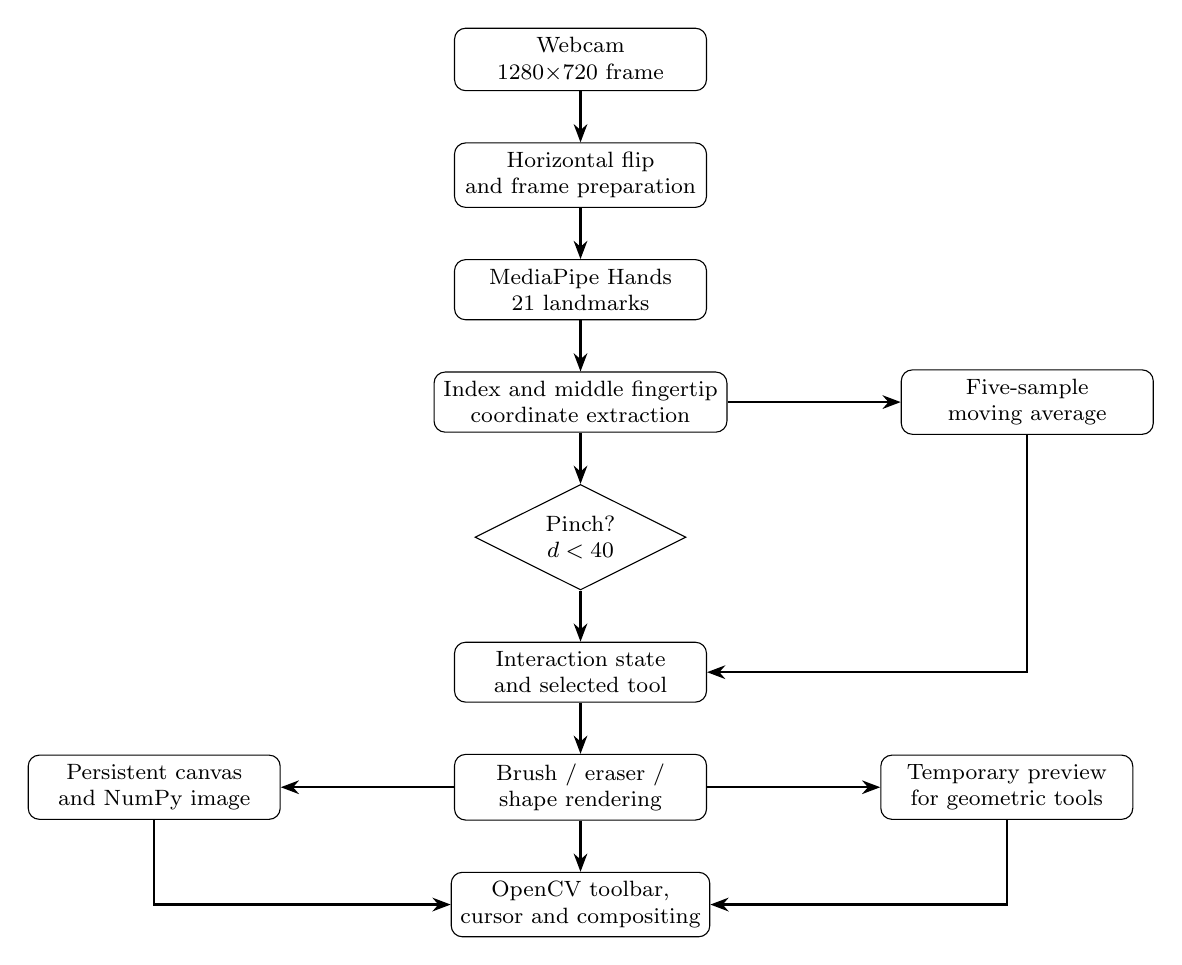
\begin{tikzpicture}[
    node distance=0.65cm,
    block/.style={
        rectangle,
        rounded corners,
        draw,
        minimum width=3.2cm,
        minimum height=0.75cm,
        align=center,
        font=\footnotesize
    },
    dec/.style={
        diamond,
        draw,
        aspect=2,
        minimum width=2.6cm,
        minimum height=0.9cm,
        align=center,
        font=\footnotesize
    },
    arrow/.style={-Stealth, thick}
]

% Main vertical pipeline
\node (cam) [block]
    {Webcam\\1280$\times$720 frame};

\node (flip) [block, below=of cam]
    {Horizontal flip\\and frame preparation};

\node (mp) [block, below=of flip]
    {MediaPipe Hands\\21 landmarks};

\node (coords) [block, below=of mp]
    {Index and middle fingertip\\coordinate extraction};

\node (pinch) [dec, below=of coords]
    {Pinch?\\$d<40$};

\node (state) [block, below=of pinch]
    {Interaction state\\and selected tool};

\node (render) [block, below=of state]
    {Brush / eraser /\\shape rendering};

% Side processing
\node (smooth) [block, right=2.2cm of coords]
    {Five-sample\\moving average};

\node (preview) [block, right=2.2cm of render]
    {Temporary preview\\for geometric tools};

\node (canvas) [block, left=2.2cm of render]
    {Persistent canvas\\and NumPy image};

\node (ui) [block, below=of render]
    {OpenCV toolbar,\\cursor and compositing};

% Main arrows
\draw[arrow] (cam) -- (flip);
\draw[arrow] (flip) -- (mp);
\draw[arrow] (mp) -- (coords);
\draw[arrow] (coords) -- (pinch);
\draw[arrow] (pinch) -- (state);
\draw[arrow] (state) -- (render);
\draw[arrow] (render) -- (ui);

% Smoothing path
\draw[arrow] (coords) -- (smooth);
\draw[arrow] (smooth) |- (state);

% Rendering branches
\draw[arrow] (render) -- (preview);
\draw[arrow] (render) -- (canvas);
\draw[arrow] (preview) |- (ui);
\draw[arrow] (canvas) |- (ui);

\end{tikzpicture}

\caption{Architecture and processing pipeline of the current AirSketch implementation.}
\label{fig:architecture}
\end{figure*}

\subsection{Fingertip Smoothing}
Raw landmark coordinates can exhibit small frame-to-frame fluctuations even when the hand is approximately stationary. Such fluctuations are undesirable for freehand drawing because they appear as unintended irregularities. AirSketch therefore stores the five most recent index-fingertip coordinates in a deque and calculates their arithmetic mean. For a window containing $N$ samples, the smoothed point is
\begin{equation}
 \bar{x}_t = \frac{1}{N}\sum_{i=0}^{N-1}x_{t-i}, \qquad
 \bar{y}_t = \frac{1}{N}\sum_{i=0}^{N-1}y_{t-i},
\end{equation}
with $N\leq5$ during startup and $N=5$ after the buffer is filled. The resulting point is rounded to an integer pixel coordinate before being used by the drawing engine. The filter is intentionally simple: it requires negligible additional computation and provides a predictable smoothing effect, although it introduces a small temporal lag compared with using the raw coordinate directly.

\subsection{Drawing State and Tool Operation}
The persistent drawing surface is a 720 by 1280 three-channel NumPy array initialized to black. A second array, `temp\_canvas`, is used for transient previews. The distinction is important for shape creation. If a user begins a rectangle, circle, line, filled rectangle, or filled circle, the system keeps the original canvas unchanged while the current pointer position is used to render a preview. Once the pinch is released, the selected primitive is drawn onto the persistent canvas.

For brush operation, consecutive fingertip positions are connected using OpenCV's line primitive. The previous coordinate is stored in `prev\_x` and `prev\_y`; the current coordinate becomes the endpoint of the next segment. This creates a continuous polyline as the hand moves. The eraser uses the same trajectory mechanism but removes previously rendered content from the canvas representation.

Geometric tools use OpenCV primitives directly. A rectangle is specified by the initial and current fingertip positions. A line uses the same pair as its endpoints. For circles, the initial position serves as the center and the Euclidean distance to the current position determines the radius:
\begin{equation}
 r = \left\lfloor\sqrt{(x_2-x_1)^2+(y_2-y_1)^2}\right\rfloor.
\end{equation}
Both outline and filled versions of rectangles and circles are available. The brush thickness is shared across drawing primitives and can take one of ten values from 5 to 50 pixels in increments of 5 pixels.

\subsection{User Interface and Control Layer}
The interface is drawn directly onto the camera frame using OpenCV. A toolbar occupies the upper part of the 1280 by 720 display, with a configured height of 82 pixels. The toolbar contains the AirSketch title, twelve color choices, eight tool buttons, and brush-size controls. Tool icons are loaded from PNG assets stored inside the project repository.

The eight available tools are brush, eraser, rectangle, circle, line, filled rectangle, filled circle, and clear canvas. Selecting a color changes the current drawing color. The brush-size section provides decrement and increment buttons and constrains the selected size to the predefined ten-value list. The clear operation replaces the persistent canvas with a new zero-valued image and resets relevant drawing state.

A hand whose smoothed fingertip lies within the toolbar region is treated as a UI interaction rather than a drawing action. The interface uses a 0.3-second debounce interval between UI interactions. This prevents repeated selections when the fingertip remains over the same button across multiple frames. The separation between toolbar and drawing region therefore forms an additional state constraint in the interaction model.

\subsection{Canvas Compositing and Display}
The drawing canvas is not displayed as a separate opaque window. Instead, the application extracts a binary mask from the current drawing image. Pixels above a grayscale threshold of 5 are treated as foreground, while the remaining pixels allow the original camera image to remain visible. The masked camera frame and masked drawing canvas are then added to produce the final composite image.

This approach creates the visual effect of drawing in the physical camera view. The fingertip cursor is rendered after the toolbar and canvas compositing, ensuring that the current interaction point remains visible above other display elements. For the eraser, the cursor preview is rendered using black rather than the current color.

\section{Implementation}

\subsection{Software Stack}
The current project is intentionally small. Its declared Python dependencies are MediaPipe 0.10.21, OpenCV 4.10.0.84, and NumPy 1.26.4 \cite{repo}. MediaPipe provides hand perception, OpenCV provides camera access, image manipulation, rendering primitives, and the desktop display loop, while NumPy provides the image-array representation used for the persistent and temporary canvases. No React, TypeScript, TensorFlow.js, Vite, Tailwind CSS, or browser canvas framework is present in the current implementation.

The source code is organized into three principal Python modules. `main.py` manages camera acquisition and the application loop. `hand\_tracker.py` encapsulates MediaPipe initialization, landmark processing, pinch detection, and fingertip smoothing. `virtual\_painter.py` maintains canvas state, tools, colors, brush size, drawing states, and frame processing. `ui.py` is responsible for toolbar rendering, icon loading, and pointer-based UI interactions. This modular separation keeps perception, drawing behavior, and presentation logic relatively independent.

\subsection{Hand Tracker Module}
The hand tracker converts each BGR frame into RGB before passing it to MediaPipe. If no hand is detected, it returns `None`, allowing the rest of the pipeline to retain the existing canvas while skipping interaction updates. When a hand is detected, MediaPipe's hand connections are rendered on the frame for visual feedback. The implementation then extracts landmarks 8 and 12 and converts their normalized coordinates to pixels.

The tracker maintains a fixed-length deque with five entries. Every valid index-fingertip position is appended, and the arithmetic mean of the available positions is returned. Because the deque is updated only when a hand is present, the filter naturally resets its effective window when tracking resumes after an absence. The current code does not perform temporal classification, velocity estimation, Kalman filtering, or adaptive thresholding.

\subsection{Virtual Painter Module}
The `VirtualPainter` object initializes the persistent canvas and temporary canvas, sets the default color and brush size, defines the available tools, and creates the hand tracker and UI objects. It also maintains the interaction state variables `drawing`, `prev\_x`, `prev\_y`, `start\_x`, and `start\_y`.

The `process\_frame` method is the central orchestration function. It first copies the persistent canvas into the temporary canvas. It then obtains hand data. If the hand is detected above the toolbar boundary, UI interaction handling takes precedence. If the hand is in the drawing region and the pinch is active, the system either starts a new interaction, extends a brush/eraser stroke, or renders a geometric preview. On pinch release, geometric tools are committed to the persistent canvas. Finally, the selected display surface is composited with the camera frame and passed to the UI renderer.

\subsection{User Interface Module}
The UI module creates the toolbar using OpenCV drawing functions. It loads the tool icons from the repository's `assets/icons` directory and supports alpha compositing for PNG images. Color selection is performed by testing the distance from the pointer to each color-circle center. Tool selection is performed by checking whether the pointer lies inside a tool button's rectangular bounds. Brush-size selection uses separate rectangular controls for decrement and increment operations.

The interface uses a 0.3-second debounce time for all UI interactions. This is a practical mechanism for reducing repeated selections caused by the high temporal sampling rate of the video stream. Importantly, the debounce applies to UI selection and not to the continuous drawing path itself, so it does not intentionally suppress ordinary brush motion.

\subsection{Interaction Mapping}
Table~\ref{tab:interaction} summarizes the current interaction model. The table distinguishes between the physical input, the interpretation performed by the software, and the resulting application behavior.

\begin{table}[t]
\caption{AirSketch Interaction Mapping}
\label{tab:interaction}
\centering
\scriptsize
\begin{tabular}{p{1.45cm}p{1.65cm}p{2.55cm}}
\toprule
\textbf{Input} & \textbf{Condition} & \textbf{System action}\\
\midrule
Index fingertip & Hand detected & Virtual pointer position\\
Index + middle tips & Distance $<40$ px & Active pinch/drawing state\\
Pinch + brush & Continuous movement & Freehand stroke\\
Pinch + eraser & Continuous movement & Blank stroke for erasing\\
Pinch + shape tool & Movement & Temporary geometric preview\\
Pinch release + shape & End of interaction & Commit shape to canvas\\
Pointer in toolbar & $y<90$ & UI interaction mode\\
Pointer on color & Within selection radius & Change drawing color\\
Pointer on tool & Within button bounds & Change active tool\\
Pointer on size control & Button bounds & Increase/decrease thickness\\
Pointer on clear & Clear button bounds & Reset persistent canvas\\
\bottomrule
\end{tabular}
\end{table}

\section{Experimental Setup and Evaluation}

\subsection{Evaluation Scope}

The current repository does not contain a formal benchmark dataset, a labeled gesture test set, or a recorded latency/accuracy measurement protocol. Consequently, this study does not report fabricated numerical recognition accuracy, latency, memory, or frame-rate results. Instead, the evaluation is framed as a functional and implementation-level assessment of the capabilities explicitly realized in the source code. This distinction is important because a working prototype and a statistically validated recognition system answer different research questions.

The implementation can nevertheless be evaluated systematically through functional scenarios. The principal scenarios are hand acquisition, fingertip tracking, pinch activation, freehand drawing, erasing, geometric shape preview and commitment, color selection, brush-size adjustment, canvas clearing, toolbar interaction, and recovery when no hand is detected. These scenarios correspond directly to the major interaction and drawing functions implemented in the current software.

\subsection{Functional Test Scenarios}

Table~\ref{tab:tests} summarizes the functional evaluation criteria used for the current implementation. A scenario is considered successful when the corresponding interaction produces the intended state transition or visual output during normal operation. The table intentionally avoids assigning unsupported percentages or numerical performance values to these observations.

\begin{table}[t]
\caption{Functional Evaluation Scenarios}
\label{tab:tests}
\centering
\scriptsize
\begin{tabular}{p{1.45cm}p{2.05cm}p{2.15cm}}
\toprule
\textbf{Scenario} & \textbf{Expected behavior} & \textbf{Implemented mechanism}\\
\midrule
Hand acquisition & Detect one hand from webcam & MediaPipe Hands, one-hand mode\\
Pointer tracking & Follow index fingertip & Landmark 8 + smoothing\\
Activation & Distinguish active input & Landmark 8--12 distance threshold\\
Freehand drawing & Produce continuous stroke & Consecutive OpenCV line segments\\
Erasing & Remove or modify drawn content & Eraser tool using fingertip interaction\\
Shape preview & Show live geometry & Temporary frame overlay\\
Shape commit & Preserve final shape & Draw on video frame at release\\
Color control & Change current color & Pointer proximity to palette\\
Tool control & Select drawing primitive & Pointer inside tool bounds\\
Size control & Adjust thickness & Bounded ten-value list\\
Clear control & Remove current drawing & Canvas/frame reset mechanism\\
No-hand state & Avoid invalid interaction & Return `None` and preserve display\\
\bottomrule
\end{tabular}
\end{table}

\subsection{Visual Output Evaluation}

Representative outputs of the AirSketch system are shown in Fig.~\ref{fig:airsketch_outputs}. The first output demonstrates the main drawing interface during operation. The webcam captures the user's hand while MediaPipe landmarks are displayed over the detected hand. The index fingertip is used as the primary interaction point for controlling drawing operations.

The output demonstrates multiple drawing capabilities within a single interaction session. Freehand strokes, a straight line, and geometric shapes are visible directly over the live video feed. The interface also provides controls for brush, eraser, line, rectangle, circle, filled rectangle, filled circle, color selection, canvas clearing, and brush-size adjustment. In the shown example, the circle tool is highlighted, demonstrating that the hand-based pointer can also be used to interact with the toolbar.

The second output demonstrates continued hand-based interaction with content already drawn on the video feed. The detected hand landmarks remain visible while the fingertip is positioned over the displayed drawing. This demonstrates that the landmark-tracking mechanism remains active while interacting with previously created visual content.

\begin{figure*}[!t]
\centering
\begin{minipage}[t]{0.48\textwidth}
    \centering
    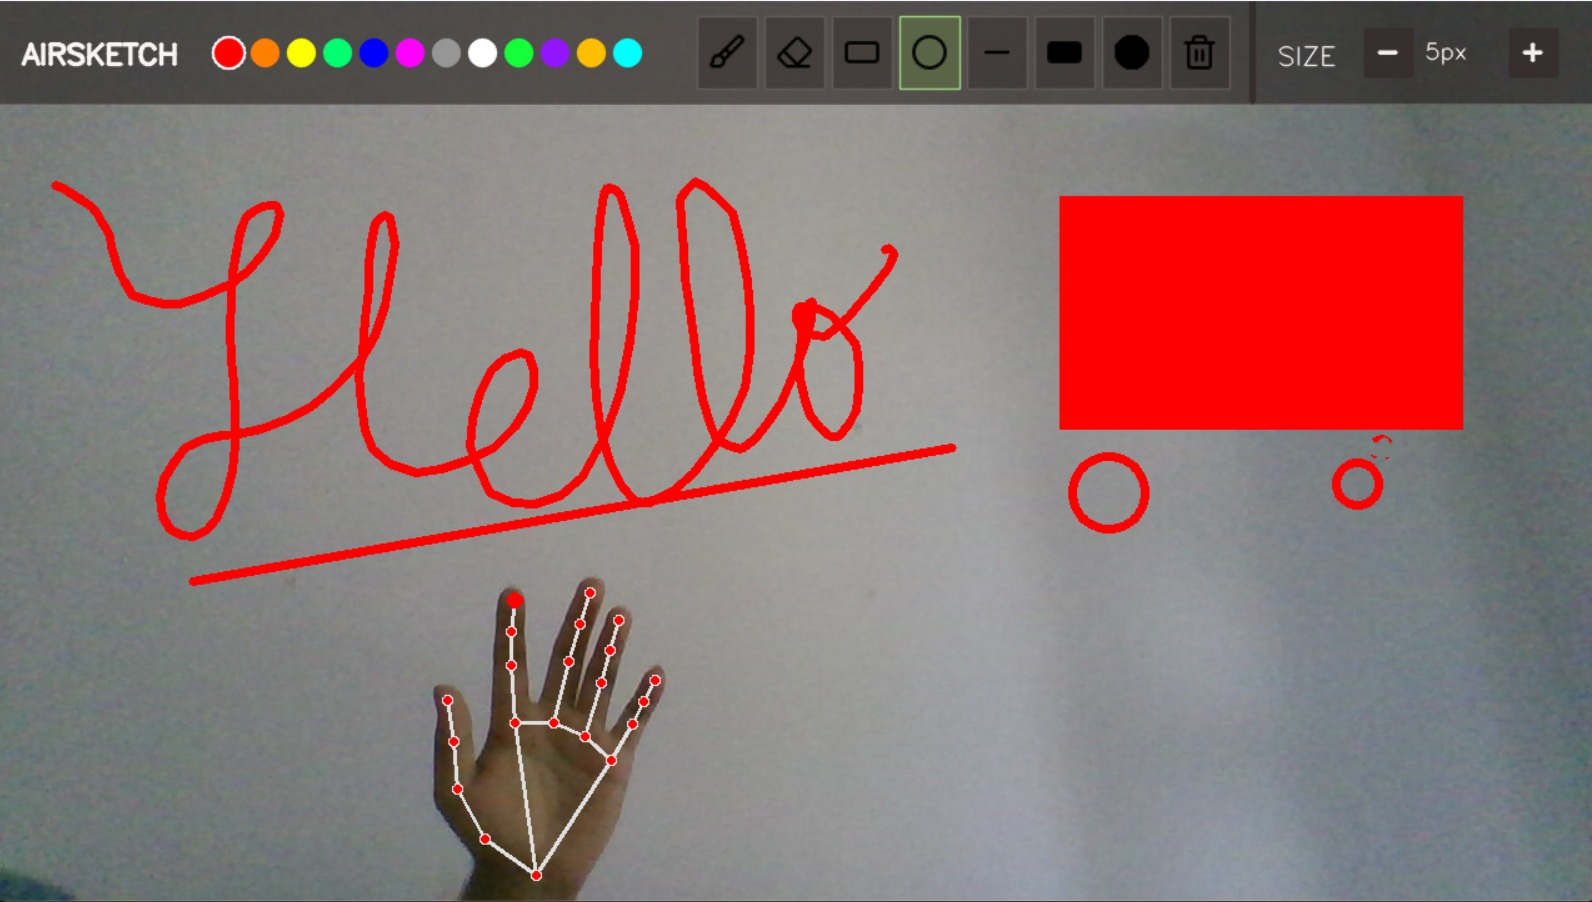
\includegraphics[width=\textwidth]{drawing_output.jpeg}
    \centerline{\footnotesize (a) Drawing and shape creation}
\end{minipage}
\hfill
\begin{minipage}[t]{0.48\textwidth}
    \centering
    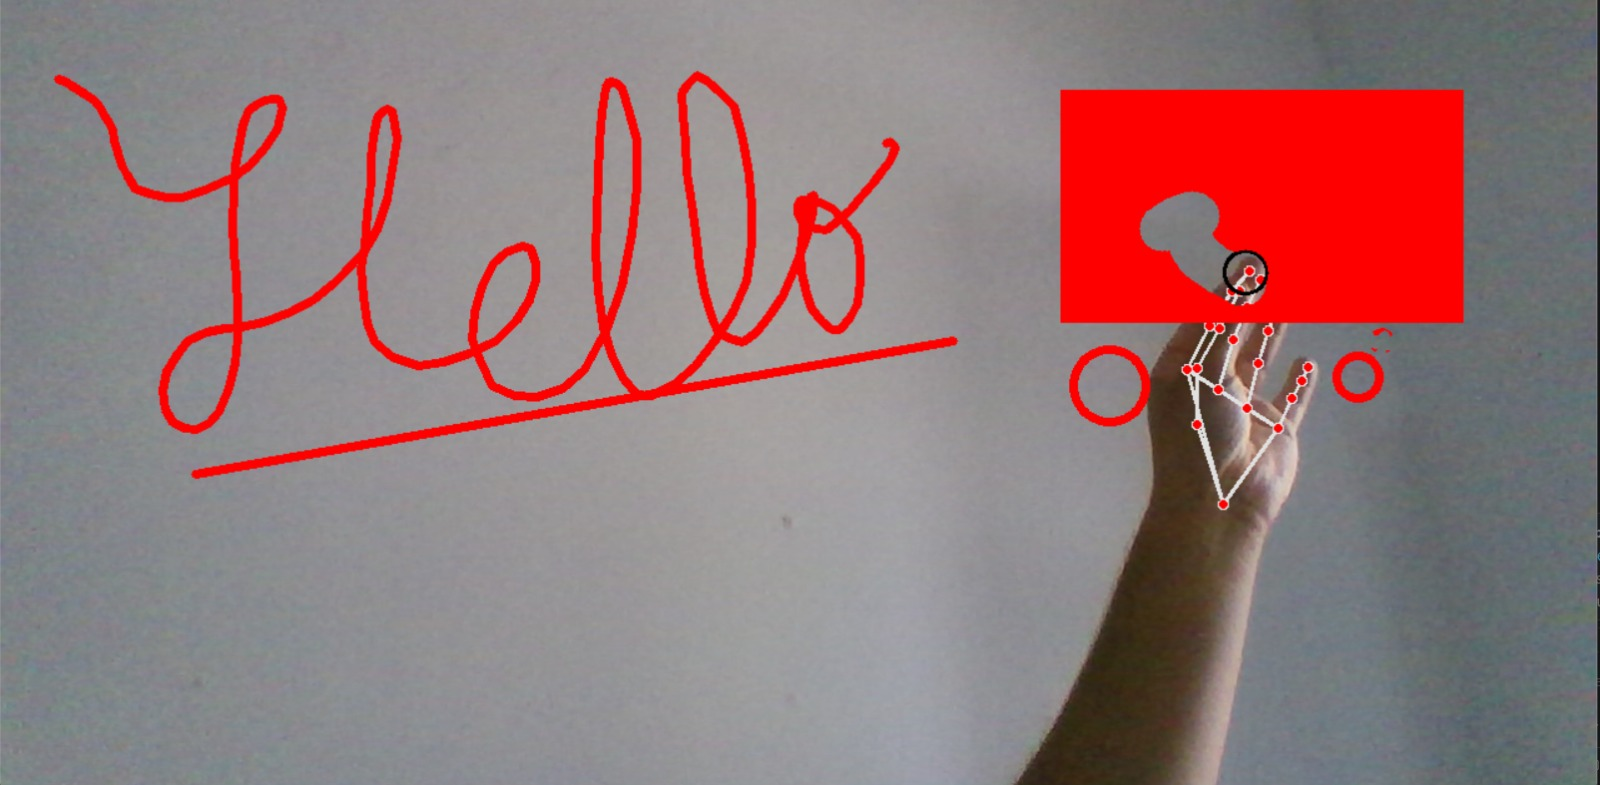
\includegraphics[width=\textwidth]{interaction_output.jpeg}
    \centerline{\footnotesize (b) Hand-based canvas interaction}
\end{minipage}
\caption{Representative AirSketch outputs demonstrating (a) freehand drawing, line and geometric shape creation with hand landmark tracking, and (b) hand-based interaction with previously drawn content directly over the live video feed.}
\label{fig:airsketch_outputs}
\end{figure*}

The displayed outputs provide functional evidence that the implemented perception and interaction pipeline can translate hand movement into drawing operations using a conventional RGB webcam. Unlike a separate black or blank drawing canvas, the current implementation renders the drawing content directly onto the live video frame, allowing the user to interact with the virtual drawing while simultaneously viewing the camera feed. However, these images represent representative functional demonstrations rather than quantitative measurements of recognition accuracy, latency, or robustness.

\subsection{Observed Interaction Characteristics}

The application performs hand tracking and drawing within the same frame-processing loop, allowing continuous interaction. The five-sample moving-average filter reduces small coordinate variations before they reach the drawing functions. For freehand tools, the drawing path is rendered incrementally using consecutive fingertip positions. For geometric tools, a temporary frame is used to preview the shape during interaction before the final geometry is committed to the displayed drawing.

The interaction model also provides a clear separation between pointer movement and activation. A user can move the fingertip without producing a new stroke when the pinch is inactive. When the pinch becomes active, the same fingertip trajectory becomes meaningful drawing input. This state-based behavior allows the user to control when a drawing operation begins and ends without requiring a physical pointing device.

The toolbar provides another level of interaction separation. When the smoothed fingertip enters the configured toolbar region, its position can be interpreted as a tool or color-selection command rather than as drawing input. The implemented debounce mechanism reduces repeated UI changes when the pointer remains over a control.

The screenshots also demonstrate that the hand-landmark visualization provides immediate feedback about the detected hand position. The user can observe the tracked hand and fingertip while drawing directly over the camera feed, providing a visual connection between physical movement and the resulting digital content.

\subsection{Discussion}

The principal strength of the current approach is that the system does not need to learn the semantics of the drawing task. MediaPipe provides a structured representation of hand geometry, after which the application applies deterministic rules. This reduces the amount of project-specific training data required and makes the control logic straightforward to explain. It also means that changing the activation rule or adding a new interaction can be done by modifying application logic rather than retraining a classifier.

The trade-off is expressiveness. A binary pinch state is sufficient for an activation mechanism but cannot by itself represent a rich vocabulary of commands. The current application therefore relies on spatial toolbar selection for tool switching instead of encoding every tool as a different hand gesture. This is a deliberate engineering choice that reduces gesture ambiguity while allowing multiple drawing operations through the same interface.

The smoothing mechanism illustrates another trade-off. A five-sample moving average is computationally inexpensive and easy to understand, but it treats recent samples uniformly and therefore does not explicitly model hand velocity or acceleration. Faster motion can consequently be smoothed less responsively than an adaptive filter would allow. Likewise, the fixed 40-pixel pinch threshold is tied to the application's pixel coordinate system rather than being normalized by hand size or camera distance. A user's apparent fingertip separation can change with distance from the camera, potentially affecting activation consistency.

Because the drawing is rendered directly onto the live video frame, the system provides an augmented camera-view interaction rather than a separate blank drawing surface. This makes the relationship between the user's physical hand movement and the resulting drawing immediately visible. However, this approach also means that the displayed drawing is dependent on the underlying video frame and the frame-compositing process.

The evaluation further highlights the practical dependence of the system on webcam quality, lighting conditions, and reliable hand visibility. The current implementation is designed for single-hand interaction and uses a fixed image-coordinate system. These factors limit the robustness of the prototype compared with systems using depth sensors or more sophisticated learned gesture models.

Overall, the functional outputs demonstrate the feasibility of using webcam-based hand landmarks and deterministic geometric interaction rules to implement a touchless virtual drawing interface directly over a live video feed. The results support the intended proof-of-concept objective of AirSketch while also identifying areas for future quantitative evaluation and robustness improvements.

\section{Limitations and Future Improvements}
Several limitations follow directly from the current implementation. First, the system processes only one detected hand. This simplifies interaction but prevents two-handed operations such as simultaneous canvas manipulation and drawing. MediaPipe itself supports multi-hand tracking, so extending the system to multiple hands is technically plausible, but the application logic would need an explicit role assignment strategy \cite{mediapipe_docs}.

Second, the system assumes a fixed 1280 by 720 coordinate space. Although MediaPipe provides normalized coordinates, the current implementation converts them directly using fixed constants. A more general implementation could derive the active dimensions from the actual captured frame, reducing dependence on camera configuration.

Third, the pinch threshold is fixed in pixels. A normalized threshold based on a scale reference such as the distance between wrist and a metacarpal landmark could make activation less sensitive to the apparent size of the hand. Such normalization would also make the interaction more transferable across camera distances.

Fourth, the current project does not use a learned gesture classifier. This is beneficial for interpretability and simplicity but limits the command vocabulary. Future versions could combine the existing landmark representation with a lightweight classifier for additional static or dynamic gestures while retaining deterministic geometric rules for core drawing operations. The literature demonstrates that landmark sequences can also be used as inputs to temporal deep-learning models for dynamic gesture recognition \cite{moreira2026,anithadevi2025}; however, adding such a model would introduce training, validation, and generalization requirements that are intentionally outside the scope of the present implementation.

Fifth, the current evaluation is functional rather than statistically controlled. A stronger experimental study should record multiple users performing repeated trials under different lighting conditions, backgrounds, camera distances, and hand orientations. Appropriate metrics could include gesture activation precision and recall, false activation rate, endpoint error, stroke deviation, task completion time, and perceived usability. Such an evaluation would allow quantitative comparison with alternative interaction mechanisms rather than relying only on implementation inspection.

Finally, the current repository creates a `paintings` directory but the inspected drawing workflow does not expose a completed image-save command. Future work can therefore add explicit save/load functionality, undo/redo operations, canvas export, and persistent project storage. Additional improvements could include adaptive stroke smoothing, normalized gesture thresholds, multi-hand support, and a richer gesture vocabulary.

\section{Conclusion}
This paper presented AirSketch, a real-time webcam-based virtual drawing and control system implemented using Python, OpenCV, MediaPipe, and NumPy. The system uses MediaPipe's 21-point hand representation to obtain fingertip positions, uses the index fingertip as a virtual pointer, and determines active interaction from the Euclidean distance between the index and middle fingertips. A five-sample moving-average filter reduces fingertip jitter before the coordinate is passed to the drawing engine.

The resulting architecture integrates freehand drawing, erasing, geometric primitives, color selection, brush-size control, and canvas clearing into a single touchless interface. Its temporary-canvas mechanism provides live previews for geometric shapes, while persistent canvas state preserves completed drawing operations. The use of deterministic landmark geometry rather than a project-specific learned classifier makes the current system lightweight and interpretable.

The analysis also shows why implementation accuracy should not be confused with benchmark accuracy. The repository supports a functional prototype with clearly defined processing and interaction rules, but it does not provide a controlled dataset or experimental measurements sufficient to justify claims such as a specific recognition percentage or end-to-end latency. A future evaluation should therefore supplement the present functional analysis with repeatable user trials and quantitative metrics.

Overall, AirSketch demonstrates that a standard webcam and a compact landmark-processing pipeline can support a practical touchless drawing interface without specialized sensing hardware. The system provides a foundation for future work involving adaptive interaction thresholds, richer gesture vocabularies, multi-hand interaction, stronger smoothing, usability studies, and persistent digital-art workflows.

\begin{thebibliography}{00}

\bibitem{zhang2020}
F. Zhang, V. Bazarevsky, A. Vakunov, A. Tkachenka, G. Sung, C.-L. Chang, and M. Grundmann, ``MediaPipe Hands: On-device Real-time Hand Tracking,'' arXiv:2006.10214, 2020.

\bibitem{qi2024}
J. Qi, L. Ma, Z. Cui, and Y. Yu, ``Computer vision-based hand gesture recognition for human-robot interaction: a review,'' \emph{Complex \& Intelligent Systems}, vol. 10, pp. 1581--1606, 2024, doi: 10.1007/s40747-023-01173-6.

\bibitem{vuletic2019}
T. Vuletic, A. Duffy, L. Hay, C. McTeague, G. Campbell, and M. Grealy, ``Systematic literature review of hand gestures used in human computer interaction interfaces,'' \emph{International Journal of Human-Computer Studies}, vol. 129, pp. 74--94, 2019, doi: 10.1016/j.ijhcs.2019.03.011.

\bibitem{rahman2020}
M. M. Rahman, M. Hossain, and M. A. H. Akhand, ``Hand Gesture Recognition Based on Computer Vision: A Review of Techniques,'' \emph{Journal of Imaging}, vol. 6, no. 8, 2020, Art. no. 73.

\bibitem{vasavi2022}
R. Vasavi, N. Rahul, A. Snigdha, K. J. Moses, and S. V. Simha, ``Painting with Hand Gestures using MediaPipe,'' \emph{International Journal of Innovative Science and Research Technology}, vol. 7, no. 12, 2022.

\bibitem{swathi2024}
S. A. Swathi, ``Air Canvas Hand Tracking,'' \emph{Journal of Emerging Technologies and Innovative Research}, vol. 11, no. 11, 2024.

\bibitem{moreira2026}
J. Moreira, ``Dynamic LIBRAS Gesture Recognition via CNN over Spatiotemporal Matrix Representation,'' arXiv:2603.25863, 2026.

\bibitem{anithadevi2025}
N. Anithadevi, S. Palanisamy, S. S. Rubini, and S. Shrestha, ``MediaPipe-LSTM-Enhanced Framework for Real-Time Dynamic Sign Language Recognition in Inclusive Communication Systems,'' \emph{Engineering Reports}, 2025.

\bibitem{mediapipe_docs}
Google AI Edge, ``MediaPipe Hands: Hand Landmark Detection,'' Google Developers, 2026. [Online]. Available: \url{https://developers.google.com/mediapipe/solutions/vision/hand_landmarker}

\bibitem{mediapipe_landmarks}
Google AI Edge, ``HandLandmark,'' Google Developers, 2026. [Online]. Available: \url{https://ai.google.dev/edge/api/mediapipe/python/mp/tasks/vision/drawing_styles/hand_landmarker/HandLandmark}

\bibitem{repo}
Code-Hish, ``MajorProject: New\_Airsketch\_Codes,'' GitHub repository, 2026. [Online]. Available: \url{https://github.com/Code-Hish/MajorProject/tree/main/New_Airsketch_Codes}

\end{thebibliography}

\end{document}
